\begin{task}
\label{TaskKW015}
\TT{Wyznacz współczynniki zespolonego szeregu Fouriera dla okresowego sygnału $f(t)$ przedstawionego na rysunku. Narysuj widmo amplitudowe i fazowe sygnału.}{Calculate coefficients of the periodic signal $f(t)$ shown below for the expansion into a complex exponential Fourier series. Draw magnitude and phase spectra.}

\begin{figure}[H]
\centering
\begin{tikzpicture}
  %\draw (0,0) circle (1in);
  \draw[->] (-3.0,+0.0) -- (+5.0,+0.0) node[right] {$t$};
  \draw[->] (+0.0,-1.5) -- (+0.0,+2.0) node[above] {$f(t)$};
  \draw[scale=1.0,domain=-1.5:-1.0,samples=100,smooth,variable=\x,red,thick] plot ({\x},{0.0+1*sin(\x*180.0/3.141592*1*3.141592/1.0)});
  \draw[-,red, thick] (-1.0,0.0) -- (0.0,0.0);
  \draw[scale=1.0,domain=0.0:1.0,samples=100,smooth,variable=\x,red,thick] plot ({\x},{0.0+1*sin(\x*180.0/3.141592*1*3.141592/1.0)});
  \draw[-,red, thick] (1.0,0.0) -- (2.0,0.0);
  \draw[scale=1.0,domain=2.0:3.0,samples=100,smooth,variable=\x,red,thick] plot ({\x},{0.0+1*sin(\x*180.0/3.141592*1*3.141592/1.0)});
  \draw[-,red, thick] (3.0,0.0) -- (3.5,0.0);
  \draw[-,red, dashed] (-2.0,1.0) -- (4.0,1.0);
  %\draw[-] (-1.0-0.1,-0.1)--(-1.0+0.1,0.1) node[midway, below, outer sep=10pt,align=center] {$-\frac{T}{2}$};
  \draw[-] (-1.0-0.1,-0.1)--(-1.0+0.1,0.1) node[midway, below, outer sep=5pt] {$-\frac{T}{2}$};
  \draw[-] (+1.0-0.1,-0.1)--(+1.0+0.1,0.1) node[midway, below, outer sep=5pt] {$\frac{T}{2}$};
  \draw[-] (+2.0-0.1,-0.1)--(+2.0+0.1,0.1) node[midway, below, outer sep=5pt] {$T$};
  \draw[-] (-0.1,+1.0-0.1)--(+0.1,+1.0+0.1) node[midway, left] {$A$};

\end{tikzpicture}
\end{figure}

\TT{W pierwszej kolejności należy ustalić wzór funkcji przedstawionej na rysunku. Jest to funkcja przedziałowa, którą możemy opisać w następujący sposób:}{First of all, the definition of $f(t)$ signal has to be derived. This is periodic piecewise function, which may be describe as:}

\begin{equation}
f(x)=\begin{cases}A \cdot sin\left( \frac{2\pi}{T} \cdot t\right) & t \in \left ( 0+k \cdot T; \frac{T}{2}+k \cdot T \right ) \\
0 & t \in \left ( \frac{T}{2}+k \cdot T; T+k \cdot T \right )\end{cases} \wedge k \in \TT{C}{Z}
\end{equation}

\TT{Współczynnik $F_0$ wyznaczamy ze wzoru:}{The $F_0$ coefficient is defined as:}

\begin{equation}
F_0=\frac{1}{T}\int_{T}f(t) \cdot dt
\end{equation}

\TT{Podstawiamy do wzoru wzór naszej funkcji w pierwszym okresie $k=0$}{For the period $t \in (0; T)$, i.e. $k=0$, we get:}

\begin{align*}
F_0&=\frac{1}{T}\int_{T}f(t) \cdot dt=\\
&=\frac{1}{T}\left(\int_{0}^{\frac{T}{2}}A \cdot sin\left( \frac{2\pi}{T} \cdot t\right) \cdot dt 
+ \frac{1}{T}\int_{\frac{T}{2}}^{T}0 \cdot dt \right)=\\
&=\frac{A}{T}\left(\int_{0}^{\frac{T}{2}}sin\left( \frac{2\pi}{T} \cdot t\right) \cdot dt 
+ 0 \right)=\\
&=\frac{A}{T}\int_{0}^{\frac{T}{2}}sin\left( \frac{2\pi}{T} \cdot t\right) \cdot dt=\\
&=\begin{Bmatrix*}[l]
z&=\frac{2\pi}{T} \cdot t\\
dz&=\frac{2\pi}{T} \cdot dt\\
dt&=\frac{dz}{\frac{2\pi}{T}}
\end{Bmatrix*}=\\
&=\frac{A}{T}\int_{0}^{\frac{T}{2}}sin\left( z\right) \cdot \frac{dz}{\frac{2\pi}{T}}=\\
&=\frac{A}{T\cdot \frac{2\pi}{T}}\int_{0}^{\frac{T}{2}}sin\left( z\right) \cdot dz=\\
&=\frac{A}{2\pi}\cdot \left(\left . -cos\left( z\right) \right|_{0}^{\frac{T}{2}}\right)=\\
&=-\frac{A}{2\pi}\cdot \left(\left . cos\left( \frac{2\pi}{T} \cdot t\right) \right|_{0}^{\frac{T}{2}}\right)=\\
&=-\frac{A}{2\pi}\cdot \left( cos\left( \frac{2\pi}{T} \cdot \frac{T}{2}\right) - cos\left( \frac{2\pi}{T} \cdot 0\right)\right)=\\
&=-\frac{A}{2\pi}\cdot \left( cos\left( \pi\right) - cos\left( 0\right)\right)=\\
&=-\frac{A}{2\pi}\cdot \left( -1 - 1\right)=\\
&=-\frac{A}{2\pi}\cdot \left( -2\right)=\\
&=\frac{A}{\pi}
\end{align*}

\TT{Wartość współczynnika $F_0$ wynosi $\frac{A}{\pi}$.}{The $F_0$ coefficient equals $\frac{A}{\pi}$.}

\TT{Współczynniki $F_k$ wyznaczamy ze wzoru}{The $F_k$ coefficients are defined as:}

\begin{equation}
F_k=\frac{1}{T}\int_{T}f(t) \cdot e^{-\jmath \cdot k \cdot \frac{2\pi}{T} \cdot t} \cdot dt
\end{equation}

\TT{Podstawiamy do wzoru wzór naszej funkcji w pierwszym okresie $k=0$}{For the period $t \in (0; T)$, i.e. $k=0$, we get:}

\begin{align*}
F_k&=\frac{1}{T}\int_{T}f(t) \cdot e^{-\jmath \cdot k \cdot \frac{2\pi}{T} \cdot t} \cdot dt=\\
&=\frac{1}{T}\cdot\left(\int_{0}^{\frac{T}{2}}A \cdot sin\left( \frac{2\pi}{T} \cdot t\right) \cdot e^{-\jmath \cdot k \cdot \frac{2\pi}{T} \cdot t} \cdot dt+\int_{\frac{T}{2}}^{T} 0 \cdot e^{-\jmath \cdot k \cdot \frac{2\pi}{T} \cdot t} \cdot dt\right)=\\
&=\frac{1}{T}\cdot\left(A \cdot \int_{0}^{\frac{T}{2}}sin\left( \frac{2\pi}{T} \cdot t\right) \cdot e^{-\jmath \cdot k \cdot \frac{2\pi}{T} \cdot t} \cdot dt+\int_{\frac{T}{2}}^{T} 0 \cdot dt\right)=\\
&=\begin{Bmatrix*}[l]
sin\left(x\right)&=\frac{e^{\jmath \cdot x}-e^{-\jmath \cdot x}}{2 \jmath }
\end{Bmatrix*}=\\
&=\frac{1}{T}\cdot\left(A \cdot \int_{0}^{\frac{T}{2}} \frac{e^{\jmath \cdot \frac{2\pi}{T} \cdot t}-e^{-\jmath \cdot \frac{2\pi}{T} \cdot t}}{2\jmath} \cdot e^{-\jmath \cdot k \cdot \frac{2\pi}{T} \cdot t} \cdot dt+0\right)=\\
&=\frac{1}{T}\cdot\left(\frac{A}{2\jmath} \cdot \int_{0}^{\frac{T}{2}} \left(e^{\jmath \cdot \frac{2\pi}{T} \cdot t}-e^{-\jmath \cdot \frac{2\pi}{T} \cdot t}\right)\cdot e^{-\jmath \cdot k \cdot \frac{2\pi}{T} \cdot t} \cdot dt\right)=\\
&=\frac{1}{T} \cdot \frac{A}{2\jmath} \cdot \int_{0}^{\frac{T}{2}}
\left( e^{\jmath \cdot \frac{2\pi}{T} \cdot t} \cdot e^{-\jmath \cdot k \cdot \frac{2\pi}{T} \cdot t} - e^{-\jmath \cdot \frac{2\pi}{T} \cdot t} \cdot e^{-\jmath \cdot k \cdot \frac{2\pi}{T} \cdot t} \right) \cdot dt=\\
&=\frac{A}{T\cdot 2\jmath} \cdot \int_{0}^{\frac{T}{2}}
\left(e^{\jmath \cdot \frac{2\pi}{T} \cdot t -\jmath \cdot k \cdot \frac{2\pi}{T} \cdot t} - e^{-\jmath \cdot \frac{2\pi}{T} \cdot t -\jmath \cdot k \cdot \frac{2\pi}{T} \cdot t} \right) \cdot dt=\\
&=\frac{A}{T\cdot 2\jmath} \cdot \int_{0}^{\frac{T}{2}}
\left(e^{\jmath \cdot \frac{2\pi}{T} \cdot t \cdot \left(1 - k\right)} - e^{-\jmath \cdot \frac{2\pi}{T} \cdot t \cdot \left(1+k\right)} \right) \cdot dt=\\
&=\frac{A}{T\cdot 2\jmath} \cdot \left( \int_{0}^{\frac{T}{2}}
e^{\jmath \cdot \frac{2\pi}{T} \cdot t \cdot \left(1 - k\right)} \cdot dt - \int_{0}^{\frac{T}{2}} e^{-\jmath \cdot \frac{2\pi}{T} \cdot t \cdot \left(1+k\right)} \cdot dt \right)=\\
&=\begin{Bmatrix*}[l]
z_1&=\jmath \cdot \frac{2\pi}{T} \cdot \left(1 - k\right)\cdot t &z_2&=-\jmath \cdot \frac{2\pi}{T} \cdot \left(1+k\right)\cdot t\\
dz_1&=\jmath \cdot \frac{2\pi}{T} \cdot \left(1 - k\right)\cdot dt &dz_2&=-\jmath \cdot \frac{2\pi}{T} \cdot \left(1+k\right)\cdot dt\\
dt&=\frac{dz_1}{\jmath \cdot \frac{2\pi}{T} \cdot \left(1 - k\right)} &dt&=\frac{dz_2}{-\jmath \cdot \frac{2\pi}{T} \cdot \left(1+k\right)}\\
\end{Bmatrix*}=\\
&=\frac{A}{T\cdot 2\jmath} \cdot \left( \int_{0}^{\frac{T}{2}}
e^{z_1} \cdot \frac{dz_1}{\jmath \cdot \frac{2\pi}{T} \cdot \left(1 - k\right)} - \int_{0}^{\frac{T}{2}} e^{z_2} \cdot \frac{dz_2}{-\jmath \cdot \frac{2\pi}{T} \cdot \left(1+k\right)} \right)=\\
&=\frac{A}{T\cdot 2\jmath} \cdot \left( \frac{1}{\jmath \cdot \frac{2\pi}{T} \cdot \left(1 - k\right)} \cdot \int_{0}^{\frac{T}{2}}
e^{z_1} \cdot dz_1 - \frac{1}{-\jmath \cdot \frac{2\pi}{T} \cdot \left(1+k\right)} \cdot \int_{0}^{\frac{T}{2}} e^{z_2} \cdot dz_2 \right)=\\
&=\frac{A}{T\cdot 2\jmath \cdot \jmath \cdot \frac{2\pi}{T} } \cdot \left( \frac{1}{1 - k} \cdot \int_{0}^{\frac{T}{2}}
e^{z_1} \cdot dz_1 + \frac{1}{1+k} \cdot \int_{0}^{\frac{T}{2}} e^{z_2} \cdot dz_2 \right)=\\
&=\frac{A}{-4 \cdot \pi} \cdot \left( \frac{1}{1 - k} \cdot \left.
e^{z_1} \right|_{0}^{\frac{T}{2}} + \frac{1}{1+k} \cdot \left. e^{z_2} \right|_{0}^{\frac{T}{2}} \right)=\\
&=\frac{A}{-4 \cdot \pi} \cdot \left( \frac{1}{1 - k} \cdot \left.
e^{\jmath \cdot \frac{2\pi}{T} \cdot \left(1 - k\right)\cdot t} \right|_{0}^{\frac{T}{2}} + \frac{1}{1+k} \cdot \left. e^{-\jmath \cdot \frac{2\pi}{T} \cdot \left(1+k\right)\cdot t} \right|_{0}^{\frac{T}{2}} \right)=\\
&=\frac{A}{-4 \cdot \pi} \cdot \left( \frac{1}{1 - k} \cdot \left(
e^{\jmath \cdot \frac{2\pi}{T} \cdot \left(1 - k\right)\cdot \frac{T}{2}} - e^{\jmath \cdot \frac{2\pi}{T} \cdot \left(1 - k\right)\cdot 0} \right) + \frac{1}{1+k} \cdot \left( e^{-\jmath \cdot \frac{2\pi}{T} \cdot \left(1+k\right)\cdot \frac{T}{2}} - e^{-\jmath \cdot \frac{2\pi}{T} \cdot \left(1+k\right)\cdot 0}\right) \right)=\\
&=\frac{A}{-4 \cdot \pi} \cdot \left( \frac{1}{1 - k} \cdot \left(
e^{\jmath \cdot \pi \cdot \left(1 - k\right)} - e^{0} \right) + \frac{1}{1+k} \cdot \left( e^{-\jmath \cdot \pi \cdot \left(1+k\right)} - e^{0}\right) \right)=\\
&=\frac{A}{-4 \cdot \pi} \cdot \left( \frac{1+k}{\left(1 - k\right)\cdot \left(1+k\right)} \cdot \left(
e^{\jmath \cdot \pi \cdot \left(1 - k\right)} - 1 \right) + \frac{1-k}{\left(1 - k\right)\cdot \left(1+k\right)} \cdot \left( e^{-\jmath \cdot \pi \cdot \left(1+k\right)} - 1\right) \right)=\\
&=\frac{A}{-4 \cdot \pi} \cdot \left( \frac{\left(1+k\right)\cdot \left(
  e^{\jmath \cdot \pi \cdot \left(1 - k\right)} - 1 \right)}{\left(1 - k\right)\cdot \left(1+k\right)} + \frac{\left(1-k\right)\cdot \left( e^{-\jmath \cdot \pi \cdot \left(1+k\right)} - 1\right)}{\left(1 - k\right)\cdot \left(1+k\right)} \right)=\\
&=\frac{A}{-4 \cdot \pi} \cdot \left( \frac{\left(1+k\right)\cdot \left(
  e^{\jmath \cdot \pi \cdot \left(1 - k\right)} - 1 \right)+\left(1-k\right)\cdot \left( e^{-\jmath \cdot \pi \cdot \left(1+k\right)} - 1\right)}{\left(1 - k\right)\cdot \left(1+k\right)} \right)=\\
&=\frac{A}{-4 \cdot \pi} \cdot \left( \frac{e^{\jmath \cdot \pi \cdot \left(1 - k\right)} - 1 + k\cdot e^{\jmath \cdot \pi \cdot \left(1 - k\right)} - k+ e^{-\jmath \cdot \pi \cdot \left(1+k\right)} - 1 - k \cdot e^{-\jmath \cdot \pi \cdot \left(1+k\right)} + k}{1-k^2} \right)=\\
&=\frac{A}{-4 \cdot \pi} \cdot \left( \frac{e^{\jmath \cdot \pi \cdot \left(1 - k\right)} - 2 + k\cdot e^{\jmath \cdot \pi \cdot \left(1 - k\right)}+ e^{-\jmath \cdot \pi \cdot \left(1+k\right)} - k \cdot e^{-\jmath \cdot \pi \cdot \left(1+k\right)}}{1-k^2} \right)=\\
&=\frac{A}{-4 \cdot \pi} \cdot \left( \frac{e^{\jmath \cdot \pi}\cdot e^{-\jmath \cdot \pi \cdot k} - 2 + k\cdot e^{\jmath \cdot \pi } \cdot e^{-\jmath \cdot \pi \cdot k}+ e^{-\jmath \cdot \pi} \cdot e^{-\jmath \cdot \pi \cdot k} - k \cdot e^{-\jmath \cdot \pi}\cdot e^{-\jmath \cdot \pi \cdot k}}{1-k^2} \right)=\\
&=\frac{A}{-4 \cdot \pi} \cdot \left( \frac{-1 \cdot e^{-\jmath \cdot \pi \cdot k} - 2 + k\cdot \left(-1\right) \cdot e^{-\jmath \cdot \pi \cdot k} -1 \cdot e^{-\jmath \cdot \pi \cdot k} - k \cdot \left(-1\right)\cdot e^{-\jmath \cdot \pi \cdot k}}{1-k^2} \right)=\\
&=\frac{A}{-4 \cdot \pi} \cdot \left( \frac{-e^{-\jmath \cdot \pi \cdot k} - 2 - k \cdot e^{-\jmath \cdot \pi \cdot k} - e^{-\jmath \cdot \pi \cdot k} + k \cdot e^{-\jmath \cdot \pi \cdot k}}{1-k^2} \right)=\\
&=\frac{A}{-4 \cdot \pi} \cdot \left( \frac{-2\cdot e^{-\jmath \cdot \pi \cdot k} - 2 }{1-k^2} \right)=\\
&=\frac{A}{4 \cdot \pi} \cdot \left( \frac{2 \cdot e^{-\jmath \cdot \pi \cdot k} +2}{1-k^2} \right)=\\
&=\frac{A}{4 \cdot \pi} \cdot 2 \cdot \left(\frac{e^{-\jmath \cdot \pi \cdot k}+1}{1-k^2} \right)=\\
&=\frac{A}{2 \cdot \pi} \cdot \left(\frac{e^{-\jmath \cdot \pi \cdot k}+1}{1-k^2}\right)\\
&=\frac{A}{2 \cdot \pi} \cdot \left(\frac{(-1)^{k}+1}{1-k^2}\right)
\end{align*}

\TT{Wartość współczynnika $F_k$ wynosi $\frac{A}{2 \cdot \pi} \cdot \left(\frac{(-1)^{k}+1}{1-k^2}\right)$ dla $k \neq 1 \wedge k \neq -1$.}{The $F_k$ coefficients equal to $\frac{A}{2 \cdot \pi} \cdot \left(\frac{(-1)^{k}+1}{1-k^2}\right)$ for $k \neq 1 \wedge k \neq -1$.}

\TT{Współczynnik $F_k$ dla $k=1$ musimy wyznaczyć raz jeszcze, tak więc wyznaczmy go wprost z definicji $F_1$:}{We have to calculate $F_k$ for $k=1$ directly by definition:}

\begin{align*}
F_1&=\frac{1}{T}\int_{T}f(t) \cdot e^{-\jmath \cdot 1 \cdot \frac{2\pi}{T} \cdot t} \cdot dt=\\
&=\frac{1}{T}\cdot\left(\int_{0}^{\frac{T}{2}}A \cdot sin\left( \frac{2\pi}{T} \cdot t\right) \cdot e^{-\jmath \cdot 1 \cdot \frac{2\pi}{T} \cdot t} \cdot dt+\int_{\frac{T}{2}}^{T} 0 \cdot e^{-\jmath \cdot 1 \cdot \frac{2\pi}{T} \cdot t} \cdot dt\right)=\\
&=\frac{1}{T}\cdot\left(A \cdot \int_{0}^{\frac{T}{2}}sin\left( \frac{2\pi}{T} \cdot t\right) \cdot e^{-\jmath \cdot \frac{2\pi}{T} \cdot t} \cdot dt+\int_{\frac{T}{2}}^{T} 0 \cdot dt\right)=\\
&=\begin{Bmatrix*}[l]
sin\left(x\right)&=\frac{e^{\jmath \cdot x}-e^{-\jmath \cdot x}}{2 \jmath }
\end{Bmatrix*}=\\
&=\frac{1}{T}\cdot\left(A \cdot \int_{0}^{\frac{T}{2}} \frac{e^{\jmath \cdot \frac{2\pi}{T} \cdot t}-e^{-\jmath \cdot \frac{2\pi}{T} \cdot t}}{2\jmath} \cdot e^{-\jmath \cdot \frac{2\pi}{T} \cdot t} \cdot dt+0\right)=\\
&=\frac{1}{T}\cdot\left(\frac{A}{2\jmath} \cdot \int_{0}^{\frac{T}{2}} \left(e^{\jmath \cdot \frac{2\pi}{T} \cdot t}-e^{-\jmath \cdot \frac{2\pi}{T} \cdot t}\right)\cdot e^{-\jmath \cdot \frac{2\pi}{T} \cdot t} \cdot dt\right)=\\
&=\frac{1}{T} \cdot \frac{A}{2\jmath} \cdot \int_{0}^{\frac{T}{2}}
\left( e^{\jmath \cdot \frac{2\pi}{T} \cdot t} \cdot e^{-\jmath \cdot \frac{2\pi}{T} \cdot t} - e^{-\jmath \cdot \frac{2\pi}{T} \cdot t} \cdot e^{-\jmath \cdot \frac{2\pi}{T} \cdot t} \right) \cdot dt=\\
&=\frac{A}{T\cdot 2\jmath} \cdot \int_{0}^{\frac{T}{2}}
\left(e^{\jmath \cdot \frac{2\pi}{T} \cdot t -\jmath \cdot \frac{2\pi}{T} \cdot t} - e^{-\jmath \cdot \frac{2\pi}{T} \cdot t -\jmath \cdot \frac{2\pi}{T} \cdot t} \right) \cdot dt=\\
&=\frac{A}{T\cdot 2\jmath} \cdot \int_{0}^{\frac{T}{2}}
\left(e^{\jmath \cdot \frac{2\pi}{T} \cdot t \cdot \left(1 - 1\right)} - e^{-\jmath \cdot \frac{2\pi}{T} \cdot t \cdot \left(1+1\right)} \right) \cdot dt=\\
&=\frac{A}{T\cdot 2\jmath} \cdot \left( \int_{0}^{\frac{T}{2}}
e^{\jmath \cdot \frac{2\pi}{T} \cdot t \cdot \left(1 - 1\right)} \cdot dt - \int_{0}^{\frac{T}{2}} e^{-\jmath \cdot \frac{2\pi}{T} \cdot t \cdot \left(1+1\right)} \cdot dt \right)=\\
&=\frac{A}{T\cdot 2\jmath} \cdot \left( \int_{0}^{\frac{T}{2}}
e^{\jmath \cdot \frac{2\pi}{T} \cdot t \cdot 0} \cdot dt - \int_{0}^{\frac{T}{2}} e^{-\jmath \cdot \frac{2\pi}{T} \cdot t \cdot 2} \cdot dt \right)=\\
&=\frac{A}{T\cdot 2\jmath} \cdot \left( \int_{0}^{\frac{T}{2}}
e^{0} \cdot dt - \int_{0}^{\frac{T}{2}} e^{-\jmath \cdot \frac{4\pi}{T} \cdot t} \cdot dt \right)=\\
&=\frac{A}{T\cdot 2\jmath} \cdot \left( \int_{0}^{\frac{T}{2}}
1 \cdot dt - \int_{0}^{\frac{T}{2}} e^{-\jmath \cdot \frac{4\pi}{T} \cdot t} \cdot dt \right)=\\
&=\begin{Bmatrix*}[l]
z&=-\jmath \cdot \frac{4\pi}{T} \cdot t\\
dz&=-\jmath \cdot \frac{4\pi}{T} \cdot dt\\
dt&=\frac{dz}{-\jmath \cdot \frac{4\pi}{T} }\\
\end{Bmatrix*}=\\
&=\frac{A}{T\cdot 2\jmath} \cdot \left( \int_{0}^{\frac{T}{2}}
dt - \int_{0}^{\frac{T}{2}} e^{z} \cdot \frac{dz}{-\jmath \cdot \frac{4\pi}{T}} \right)=\\
&=\frac{A}{T\cdot 2\jmath} \cdot \left( \int_{0}^{\frac{T}{2}}
dt - \frac{1}{-\jmath \cdot \frac{4\pi}{T}} \cdot \int_{0}^{\frac{T}{2}} e^{z} \cdot dz \right)=\\
&=\frac{A}{T\cdot 2\jmath} \cdot \left(\left. t \right|_{0}^{\frac{T}{2}} + \frac{1}{\jmath \cdot \frac{4\pi}{T}} \cdot \left. e^{z} \right|_{0}^{\frac{T}{2}} \right)=\\
&=\frac{A}{T\cdot 2\jmath} \cdot \left(\left( \frac{T}{2}- 0 \right) + \frac{1}{\jmath \cdot \frac{4\pi}{T}} \cdot \left. e^{-\jmath \cdot \frac{4\pi}{T} \cdot t} \right|_{0}^{\frac{T}{2}} \right)=\\
&=\frac{A}{T\cdot 2\jmath} \cdot \left(\left( \frac{T}{2}- 0 \right) + \frac{1}{\jmath \cdot \frac{4\pi}{T}} \cdot \left( e^{-\jmath \cdot \frac{4\pi}{T} \cdot \frac{T}{2}} - e^{-\jmath \cdot \frac{4\pi}{T} \cdot 0}\right)\right)=\\
&=\frac{A}{T\cdot 2\jmath} \cdot \left( \frac{T}{2} + \frac{1}{\jmath \cdot \frac{4\pi}{T}} \cdot \left( e^{-\jmath \cdot 2\pi} - e^{0}\right)\right)=\\
&=\frac{A}{T\cdot 2\jmath} \cdot \left( \frac{T}{2} + \frac{1}{\jmath \cdot \frac{4\pi}{T}} \cdot \left( 1 - 1\right)\right)=\\
&=\frac{A}{T\cdot 2\jmath} \cdot \left( \frac{T}{2} + \frac{1}{\jmath \cdot \frac{4\pi}{T}} \cdot 0\right)=\\
&=\frac{A}{T\cdot 2\jmath} \cdot \left( \frac{T}{2} + 0\right)=\\
&=\frac{A}{T\cdot 2\jmath} \cdot \frac{T}{2} =\\
&=\frac{A}{4 \jmath} =\\
&=-\jmath \cdot \frac{A}{4}
\end{align*}

\TT{Wartość współczynnika $F_1$ wynosi $-\jmath \cdot \frac{A}{4}$.}{The $F_1$ coefficients equal to $-\jmath \cdot \frac{A}{4}$.}

\TT{Współczynnik $F_k$ dla $k=-1$ musimy wyznaczyć raz jeszcze, tak więc wyznaczmy go wprost z definicji $F_{-1}$:}{We have to calculate $F_k$ for $k=-1$ directly by definition:}

\begin{align*}
F_{-1}&=\frac{1}{T}\int_{T}f(t) \cdot e^{-\jmath \cdot (-1) \cdot \frac{2\pi}{T} \cdot t} \cdot dt=\\
&=\frac{1}{T}\cdot\left(\int_{0}^{\frac{T}{2}}A \cdot sin\left( \frac{2\pi}{T} \cdot t\right) \cdot e^{-\jmath \cdot (-1) \cdot \frac{2\pi}{T} \cdot t} \cdot dt+\int_{\frac{T}{2}}^{T} 0 \cdot e^{-\jmath \cdot (-1) \cdot \frac{2\pi}{T} \cdot t} \cdot dt\right)=\\
&=\frac{1}{T}\cdot\left(A \cdot \int_{0}^{\frac{T}{2}}sin\left( \frac{2\pi}{T} \cdot t\right) \cdot e^{\jmath \cdot \frac{2\pi}{T} \cdot t} \cdot dt+\int_{\frac{T}{2}}^{T} 0 \cdot dt\right)=\\
&=\begin{Bmatrix*}[l]
sin\left(x\right)&=\frac{e^{\jmath \cdot x}-e^{-\jmath \cdot x}}{2 \jmath }
\end{Bmatrix*}=\\
&=\frac{1}{T}\cdot\left(A \cdot \int_{0}^{\frac{T}{2}} \frac{e^{\jmath \cdot \frac{2\pi}{T} \cdot t}-e^{-\jmath \cdot \frac{2\pi}{T} \cdot t}}{2\jmath} \cdot e^{\jmath \cdot \frac{2\pi}{T} \cdot t} \cdot dt+0\right)=\\
&=\frac{1}{T}\cdot\left(\frac{A}{2\jmath} \cdot \int_{0}^{\frac{T}{2}} \left(e^{\jmath \cdot \frac{2\pi}{T} \cdot t}-e^{-\jmath \cdot \frac{2\pi}{T} \cdot t}\right)\cdot e^{\jmath \cdot \frac{2\pi}{T} \cdot t} \cdot dt\right)=\\
&=\frac{1}{T} \cdot \frac{A}{2\jmath} \cdot \int_{0}^{\frac{T}{2}}
\left( e^{\jmath \cdot \frac{2\pi}{T} \cdot t} \cdot e^{\jmath \cdot \frac{2\pi}{T} \cdot t} - e^{-\jmath \cdot \frac{2\pi}{T} \cdot t} \cdot e^{\jmath \cdot \frac{2\pi}{T} \cdot t} \right) \cdot dt=\\
&=\frac{A}{T\cdot 2\jmath} \cdot \int_{0}^{\frac{T}{2}}
\left(e^{\jmath \cdot \frac{2\pi}{T} \cdot t +\jmath \cdot \frac{2\pi}{T} \cdot t} - e^{-\jmath \cdot \frac{2\pi}{T} \cdot t +\jmath \cdot \frac{2\pi}{T} \cdot t} \right) \cdot dt=\\
&=\frac{A}{T\cdot 2\jmath} \cdot \int_{0}^{\frac{T}{2}}
\left(e^{\jmath \cdot \frac{2\pi}{T} \cdot t \cdot \left(1 + 1\right)} - e^{-\jmath \cdot \frac{2\pi}{T} \cdot t \cdot \left(1-1\right)} \right) \cdot dt=\\
&=\frac{A}{T\cdot 2\jmath} \cdot \left( \int_{0}^{\frac{T}{2}}
e^{\jmath \cdot \frac{2\pi}{T} \cdot t \cdot \left(1 + 1\right)} \cdot dt - \int_{0}^{\frac{T}{2}} e^{-\jmath \cdot \frac{2\pi}{T} \cdot t \cdot \left(1-1\right)} \cdot dt \right)=\\
&=\frac{A}{T\cdot 2\jmath} \cdot \left( \int_{0}^{\frac{T}{2}}
e^{\jmath \cdot \frac{2\pi}{T} \cdot t \cdot 2} \cdot dt - \int_{0}^{\frac{T}{2}} e^{-\jmath \cdot \frac{2\pi}{T} \cdot t \cdot 0} \cdot dt \right)=\\
&=\frac{A}{T\cdot 2\jmath} \cdot \left( \int_{0}^{\frac{T}{2}} e^{\jmath \cdot \frac{4\pi}{T} \cdot t} \cdot dt - \int_{0}^{\frac{T}{2}}
e^{0} \cdot dt \right)=\\
&=\frac{A}{T\cdot 2\jmath} \cdot \left(\int_{0}^{\frac{T}{2}} e^{\jmath \cdot \frac{4\pi}{T} \cdot t} \cdot dt - \int_{0}^{\frac{T}{2}}
1 \cdot dt\right)=\\
&=\begin{Bmatrix*}[l]
z&=\jmath \cdot \frac{4\pi}{T} \cdot t\\
dz&=\jmath \cdot \frac{4\pi}{T} \cdot dt\\
dt&=\frac{dz}{\jmath \cdot \frac{4\pi}{T} }\\
\end{Bmatrix*}=\\
&=\frac{A}{T\cdot 2\jmath} \cdot \left( \int_{0}^{\frac{T}{2}} e^{z} \cdot \frac{dz}{\jmath \cdot \frac{4\pi}{T}} - \int_{0}^{\frac{T}{2}}
dt \right)=\\
&=\frac{A}{T\cdot 2\jmath} \cdot \left(\frac{1}{\jmath \cdot \frac{4\pi}{T}} \cdot \int_{0}^{\frac{T}{2}} e^{z} \cdot dz - \int_{0}^{\frac{T}{2}}
dt \right)=\\
&=\frac{A}{T\cdot 2\jmath} \cdot \left(\frac{1}{\jmath \cdot \frac{4\pi}{T}} \cdot \left. e^{z} \right|_{0}^{\frac{T}{2}} - \left. t \right|_{0}^{\frac{T}{2}} \right)=\\
&=\frac{A}{T\cdot 2\jmath} \cdot \left(\frac{1}{\jmath \cdot \frac{4\pi}{T}} \cdot \left. e^{-\jmath \cdot \frac{4\pi}{T} \cdot t} \right|_{0}^{\frac{T}{2}} - \left( \frac{T}{2}- 0 \right) \right)=\\
&=\frac{A}{T\cdot 2\jmath} \cdot \left( \frac{1}{\jmath \cdot \frac{4\pi}{T}} \cdot \left( e^{-\jmath \cdot \frac{4\pi}{T} \cdot \frac{T}{2}} - e^{-\jmath \cdot \frac{4\pi}{T} \cdot 0}\right) - \left( \frac{T}{2}- 0 \right) \right)=\\
&=\frac{A}{T\cdot 2\jmath} \cdot \left( \frac{1}{\jmath \cdot \frac{4\pi}{T}} \cdot \left( e^{-\jmath \cdot 2\pi} - e^{0}\right) - \frac{T}{2}\right)=\\
&=\frac{A}{T\cdot 2\jmath} \cdot \left( \frac{1}{\jmath \cdot \frac{4\pi}{T}} \cdot \left( 1 - 1\right) - \frac{T}{2}\right)=\\
&=\frac{A}{T\cdot 2\jmath} \cdot \left( \frac{1}{\jmath \cdot \frac{4\pi}{T}} \cdot 0 - \frac{T}{2}\right)=\\
&=\frac{A}{T\cdot 2\jmath} \cdot \left( 0 - \frac{T}{2}\right)=\\
&=-\frac{A}{T\cdot 2\jmath} \cdot \frac{T}{2} =\\
&=-\frac{A}{4 \jmath} =\\
&=\jmath \cdot \frac{A}{4} 
\end{align*}

\TT{Wartość współczynnika $F_{-1}$ wynosi $\jmath \cdot \frac{A}{4}$.}{The $F_{-1}$ coefficients equal to $\jmath \cdot \frac{A}{4}$.}

\TT{Ostatecznie współczynniki zespolonego szeregu Fouriera dla funkcji przedstawionej na rysunku przyjmują wartości.}{To sum up, coefficients for the expansion into a complex exponential Fourier series are given by:}

\begin{align*}
F_0&=\frac{A}{\pi}\\
F_{-1}&=\jmath \cdot \frac{A}{4}\\
F_{1}&=-\jmath \cdot \frac{A}{4}\\
F_k&=\frac{A}{2 \cdot \pi} \cdot \left(\frac{(-1)^{k}+1}{1-k^2}\right)\\
\end{align*}

\TT{Podstawiając to wzoru aproksymacyjnego funkcję $f(t)$ możemy wyrazić jako}{Hence, the signal $f(t)$ may be expressed as the sum of the harmonic series}

\begin{equation}
\begin{aligned}
f(t) &= \sum_{k=-\infty}^{\infty} F_k \cdot e^{\jmath \cdot k \cdot \frac{2\pi}{T} \cdot t}\\
f(t) &= \frac{A}{\pi} + \jmath \cdot \frac{A}{4} \cdot e^{\jmath \cdot (-1) \cdot \frac{2\pi}{T} \cdot t} - \jmath \cdot \frac{A}{4} \cdot e^{\jmath \cdot 1 \cdot \frac{2\pi}{T} \cdot t} + \sum_{\begin{smallmatrix}k=-\infty \\ k \neq 0 \\ k \neq -1 \wedge k \neq 1 \end{smallmatrix}}^{\infty} \left[\frac{A}{2 \cdot \pi} \cdot \left(\frac{(-1)^{k}+1}{1-k^2}\right)\right] \cdot e^{\jmath \cdot k \cdot \frac{2\pi}{T} \cdot t}
\end{aligned}
\end{equation}

\TT{Możemy wyznaczyć kilka wartości współczynników $F_k$}{The first several coefficients are equal to:}

\begin{table}[H]
  \centering  
  \begin{tabular}{|c|c|c|c|c|c|c|c|c|c|c|c|c|c|}
    \hline 
    $F_k$ & $-6$ & $-5$ & $-4$ & $-3$ & $-2$ & $-1$ & $0$& $1$& $2$& $3$& $4$& $5$ & $6$\\ 
    \hline 
    $F_k$ & $-\frac{A}{35\pi}$ & $0$ & $-\frac{A}{15\pi}$ & $0$ & $-\frac{A}{3\pi}$ & $\jmath \cdot \frac{A}{4}$ & $\frac{A}{\pi}$ & $-\jmath \cdot \frac{A}{4}$ & $-\frac{A}{3\pi}$ & $0$ & $-\frac{A}{15\pi}$ & $0$ & $-\frac{A}{35\pi}$\\ 
    \hline 
    $\left|F_k\right|$ & $\frac{A}{35\pi}$ & $0$ & $\frac{A}{15\pi}$ & $0$ & $\frac{A}{3\pi}$ & $\frac{A}{4}$ & $\frac{A}{\pi}$ & $\frac{A}{4}$ & $\frac{A}{3\pi}$ & $0$ & $\frac{A}{15\pi}$ & $0$ & $\frac{A}{35\pi}$\\ 
    \hline
    $Arg\left\{ F_k \right\}$ & $-\pi$ & $0$ & $-\pi$ & $0$ & $-\pi$ & $\frac{\pi}{2}$ & $0$ & -$\frac{\pi}{2}$ & $\pi$ & $0$ & $\pi$ & $0$ & $\pi$\\
    \hline 
  \end{tabular} 
\end{table}

\TT{Na podstawie wyznaczonych współczynników $F_k$ możemy narysować widmo amplitudowe $\left|F_k\right|$ sygnału $f(t)$.}{Based on coefficents $F_k$ we can plot magnitude spectrum $\left|F_k\right|$ of the $f(t)$ signal.}

\begin{figure}[H]
    \centering
    \begin{tikzpicture}
    
    \tikzmath{
        function mFk(\k,\A) {
            if(\k==0) then
            {
                return \A/3.141592;
            }
            else
            {
                if(\k==1) then 
                {
                    return \A/4;
                }
                else
                {
                    if(\k==-1) then
                    {
                        return \A/4;
                    }
                    else
                    {
                        %return abs(\A/(2*3.141592)*(sqrt((cos(\k*180)+1.0)^2+(sin(-\k*180))^2) )/(1-(\k)^2));
                        return abs(\A/(2*3.141592)*(((-1)^\k) + 1)/(1-(\k)^2));
                    };
                };        
            };
        };
    }
    
    %\draw (0,0) circle (1in);
    \draw[->] (-6.0,+0.0) -- (+6.0,+0.0) node[right] {$k$};
    \draw[->] (+0.0,-0.0) -- (+0.0,+2.5) node[above] {$\left|F_k\right|$};
    \draw[-] (-0.1,2.0-0.1)--(+0.1,2.0+0.1) node[midway, left] {$A/\pi$};
    
    \foreach \k in {-8,-7,...,8 }{
        \pgfmathsetmacro{\x}{\k/1.5};
        \draw[-] ({\x-0.1},-0.1)--({\x+0.1},0.1) node[midway, below, outer sep=5pt] {${\k}$};    
    };
    
    \foreach \k in {-8,-7,...,8 }{
        \pgfmathsetmacro{\x}{\k/1.5};
        \pgfmathsetmacro{\y}{mFk(\k,4)*3.141592/2.0};
        \node[circle,red,fill=red,scale=0.5] (\x\y) at (\x,\y) {};
        \draw[-, red] (\x,0) -- (\x,\y);
    };
    
    \end{tikzpicture}
\end{figure}

\TT{Widmo aplitudowe sygnału rzeczywistego jest zawsze parzyste.}{The magnitude spectrum of a \underline{real signal} is an even-symmetric function of $k$.}

\TT{Podobnie n podstawie wyznaczonych współczynników $F_k$ możemy narysować widmo fazowe $\mathtt{arg}\left\{F_k\right\}$ sygnału $f(t)$.}{Based on coefficents $F_k$ we can plot phase spectrum $\mathtt{arg}\left\{F_k\right\}$ of the $f(t)$ signal.}

\begin{figure}[H]
    \centering
    \begin{tikzpicture}
    
    \tikzmath{
        function aFk(\k,\A) {
            if(\k==0) then
            {
                return 0;
            }
            else
            {
                if(\k==1) then 
                {
                    return -3.141592/2;
                }
                else
                {
                    if(\k==-1) then
                    {
                        return 3.141592/2;
                    }
                    else
                    {
                        if(mod(abs(\k),2))==1) then
                        {
                            return 0; % odd
                        }
                        else
                        {
                            return 3.141592*sign(\k); %even * sign
                        };
                    };
                };
            };
        };
    }
    
    %\draw (0,0) circle (1in);
    \draw[->] (-6.0,+0.0) -- (+6.0,+0.0) node[right] {$k$};
    \draw[->] (+0.0,-2.5) -- (+0.0,+2.5) node[above] {$\mathtt{arg}\left\{F_k\right\}$};
    \draw[-] (-0.1,2.0-0.1)--(+0.1,2.0+0.1) node[midway, left] {$\pi$};
    \draw[-] (-0.1,-2.0-0.1)--(+0.1,-2.0+0.1) node[midway, left] {$-\pi$};
    \draw[-] (-0.1,1.0-0.1)--(+0.1,1.0+0.1) node[midway, left] {$\frac{\pi}{2}$};
    \draw[-] (-0.1,-1.0-0.1)--(+0.1,-1.0+0.1) node[midway, left] {$-\frac{\pi}{2}$};
    
    \foreach \k in {-8,-7,...,8 }{
        \pgfmathsetmacro{\x}{\k/1.5};
        \draw[-] ({\x-0.1},-0.1)--({\x+0.1},0.1) node[midway, below, outer sep=5pt] {${\k}$};    
    };
    
    \foreach \k in {-8,-7,...,8 }{
        \pgfmathsetmacro{\x}{\k/1.5};
        \pgfmathsetmacro{\y}{aFk(\k,4)*2.0/3.141592};
        \node[circle,red,fill=red,scale=0.5] (\x\y) at (\x,\y) {};
        \draw[-, red] (\x,0) -- (\x,\y);
    };
    
    \end{tikzpicture}
\end{figure}

\TT{Widmo fazowe sygnału rzeczywistego jest zawsze nieparzyste.}{The phase spectrum of a \underline{real signal} is an odd-symmetric function of $k$.}

\TT{W przypadku sumowania od $k_{min}=-1$ do $k_{max}=1$ otrzymujemy:}{A partial approximation of the $f(t)$ signal from $k_{min}=-1$ to $k_{max}=1$ results in:}

\begin{figure}[H]
  \centering
  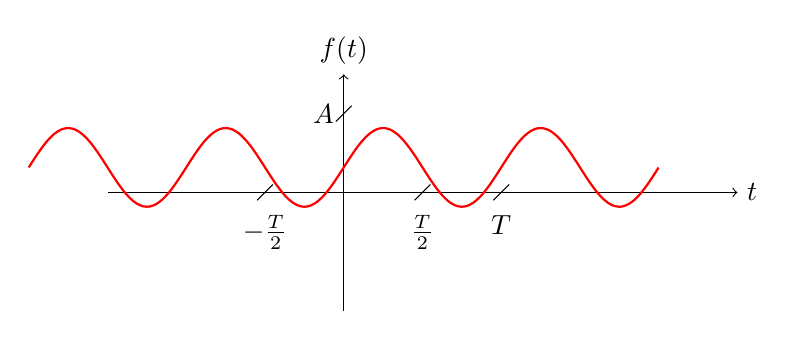
\begin{tikzpicture}
  %\draw (0,0) circle (1in);
  \draw[->] (-3.0,+0.0) -- (+5.0,+0.0) node[right] {$t$};
  \draw[->] (+0.0,-1.5) -- (+0.0,+1.5) node[above] {$f(t)$};
  %\draw[-,red, thick] (-2.5,+0.0) -- (+0.0,+0.0);
  %\draw[-] (-1.0-0.1,-0.1)--(-1.0+0.1,0.1) node[midway, below, outer sep=10pt,align=center] {$-\frac{T}{2}$};
  \draw[-] (-1.0-0.1,-0.1)--(-1.0+0.1,0.1) node[midway, below, outer sep=5pt,align=center] {$-\frac{T}{2}$};
  \draw[-] (+1.0-0.1,-0.1)--(+1.0+0.1,0.1) node[midway, below, outer sep=5pt] {$\frac{T}{2}$};
  \draw[-] (+2.0-0.1,-0.1)--(+2.0+0.1,0.1) node[midway, below, outer sep=5pt] {$T$};
  \draw[-] (-0.1,1.0-0.1)--(+0.1,1.0+0.1) node[midway, left] {$A$};
  
  \draw[scale=1.0,domain=-4:4.0,samples=100,smooth,variable=\x,red,thick] plot ({\x},{1.0/3.141592+1.0/2.0*sin(\x*180.0/3.141592*1.0*3.141592/1.0)});
  \end{tikzpicture}
\end{figure}

\TT{W przypadku sumowania od $k_{min}=-2$ do $k_{max}=2$ otrzymujemy:}{A partial approximation of the $f(t)$ signal from $k_{min}=-2$ to $k_{max}=2$ results in:}

\begin{figure}[H]
  \centering
  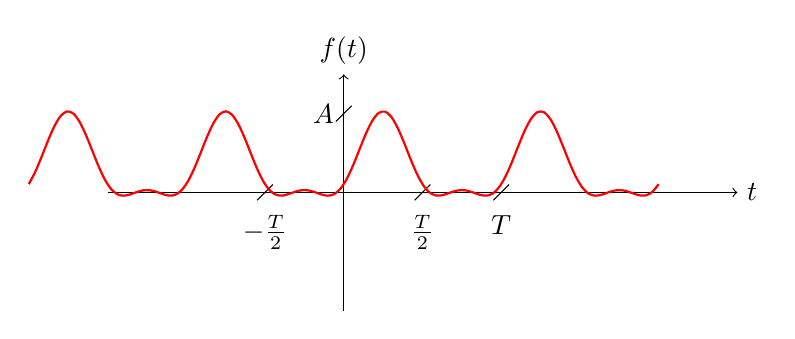
\begin{tikzpicture}
  %\draw (0,0) circle (1in);
  \draw[->] (-3.0,+0.0) -- (+5.0,+0.0) node[right] {$t$};
  \draw[->] (+0.0,-1.5) -- (+0.0,+1.5) node[above] {$f(t)$};
  %\draw[-,red, thick] (-2.5,+0.0) -- (+0.0,+0.0);
  %\draw[-] (-1.0-0.1,-0.1)--(-1.0+0.1,0.1) node[midway, below, outer sep=10pt,align=center] {$-\frac{T}{2}$};
  \draw[-] (-1.0-0.1,-0.1)--(-1.0+0.1,0.1) node[midway, below, outer sep=5pt,align=center] {$-\frac{T}{2}$};
  \draw[-] (+1.0-0.1,-0.1)--(+1.0+0.1,0.1) node[midway, below, outer sep=5pt] {$\frac{T}{2}$};
  \draw[-] (+2.0-0.1,-0.1)--(+2.0+0.1,0.1) node[midway, below, outer sep=5pt] {$T$};
  \draw[-] (-0.1,1.0-0.1)--(+0.1,1.0+0.1) node[midway, left] {$A$};
  
  \draw[scale=1.0,domain=-4:4.0,samples=100,smooth,variable=\x,red,thick] plot ({\x},{1.0/3.141592+1.0/2.0*sin(\x*180.0/3.141592*1.0*3.141592/1.0)-2.0/(3.0*3.141592)*cos(\x*180.0/3.141592*2.0*3.141592/1.0)});
  \end{tikzpicture}
\end{figure}

\TT{W przypadku sumowania od $k_{min}=-4$ do $k_{max}=4$ otrzymujemy:}{A partial approximation of the $f(t)$ signal from $k_{min}=-4$ to $k_{max}=4$ results in:}

\begin{figure}[H]
  \centering
  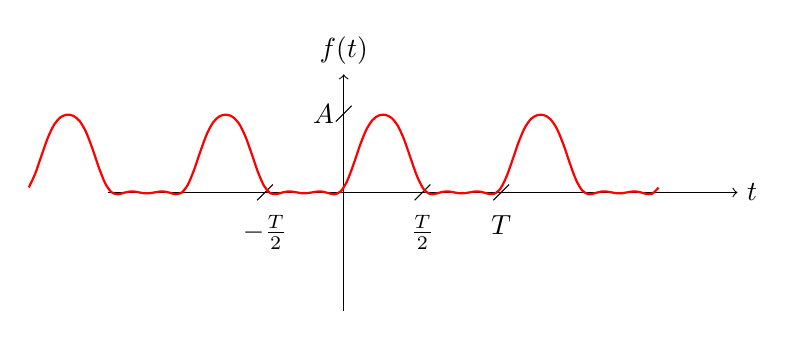
\begin{tikzpicture}
  %\draw (0,0) circle (1in);
  \draw[->] (-3.0,+0.0) -- (+5.0,+0.0) node[right] {$t$};
  \draw[->] (+0.0,-1.5) -- (+0.0,+1.5) node[above] {$f(t)$};
  %\draw[-,red, thick] (-2.5,+0.0) -- (+0.0,+0.0);
  %\draw[-] (-1.0-0.1,-0.1)--(-1.0+0.1,0.1) node[midway, below, outer sep=10pt,align=center] {$-\frac{T}{2}$};
  \draw[-] (-1.0-0.1,-0.1)--(-1.0+0.1,0.1) node[midway, below, outer sep=5pt,align=center] {$-\frac{T}{2}$};
  \draw[-] (+1.0-0.1,-0.1)--(+1.0+0.1,0.1) node[midway, below, outer sep=5pt] {$\frac{T}{2}$};
  \draw[-] (+2.0-0.1,-0.1)--(+2.0+0.1,0.1) node[midway, below, outer sep=5pt] {$T$};
  \draw[-] (-0.1,1.0-0.1)--(+0.1,1.0+0.1) node[midway, left] {$A$};
  
  \draw[scale=1.0,domain=-4:4.0,samples=100,smooth,variable=\x,red,thick] plot ({\x},{1.0/3.141592+1.0/2.0*sin(\x*180.0/3.141592*1*3.141592/1.0)-2.0/(3.0*3.141592)*cos(\x*180.0/3.141592*2.0*3.141592/1.0)-2.0/(15.0*3.141592)*cos(\x*180.0/3.141592*4.0*3.141592/1.0)});
  \end{tikzpicture}
\end{figure}

\TT{W przypadku sumowania od $k_{min}=-6$ do $k_{max}=6$ otrzymujemy:}{A partial approximation of the $f(t)$ signal from $k_{min}=-6$ to $k_{max}=6$ results in:}

\begin{figure}[H]
  \centering
  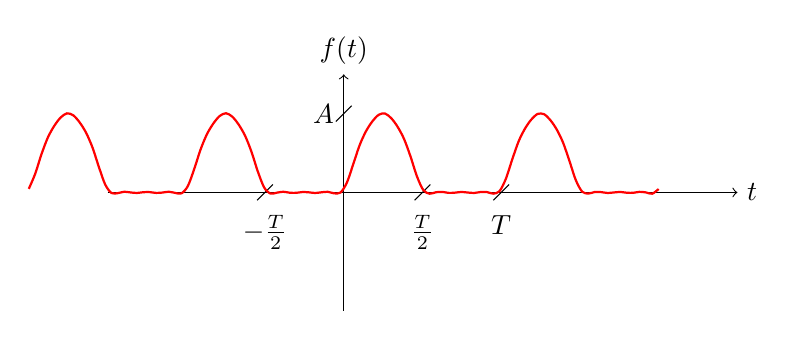
\begin{tikzpicture}
  %\draw (0,0) circle (1in);
  \draw[->] (-3.0,+0.0) -- (+5.0,+0.0) node[right] {$t$};
  \draw[->] (+0.0,-1.5) -- (+0.0,+1.5) node[above] {$f(t)$};
  %\draw[-,red, thick] (-2.5,+0.0) -- (+0.0,+0.0);
  %\draw[-] (-1.0-0.1,-0.1)--(-1.0+0.1,0.1) node[midway, below, outer sep=10pt,align=center] {$-\frac{T}{2}$};
  \draw[-] (-1.0-0.1,-0.1)--(-1.0+0.1,0.1) node[midway, below, outer sep=5pt,align=center] {$-\frac{T}{2}$};
  \draw[-] (+1.0-0.1,-0.1)--(+1.0+0.1,0.1) node[midway, below, outer sep=5pt] {$\frac{T}{2}$};
  \draw[-] (+2.0-0.1,-0.1)--(+2.0+0.1,0.1) node[midway, below, outer sep=5pt] {$T$};
  \draw[-] (-0.1,1.0-0.1)--(+0.1,1.0+0.1) node[midway, left] {$A$};
  
  \draw[scale=1.0,domain=-4:4.0,samples=100,smooth,variable=\x,red,thick] plot ({\x},{1.0/3.141592+1.0/2.0*sin(\x*180.0/3.141592*1*3.141592/1.0)-2.0/(3.0*3.141592)*cos(\x*180.0/3.141592*2.0*3.141592/1.0)-2.0/(15.0*3.141592)*cos(\x*180.0/3.141592*4.0*3.141592/1.0)-2.0/(35.0*3.141592)*cos(\x*180.0/3.141592*6.0*3.141592/1.0)});
  \end{tikzpicture}
\end{figure}

\TT{W przypadku sumowania od $k_{min}=-12$ do $k_{max}=12$ otrzymujemy:}{A partial approximation of the $f(t)$ signal from $k_{min}=-12$ to $k_{max}=12$ results in:} 

\begin{figure}[H]
  \centering
  \begin{tikzpicture}
  %\draw (0,0) circle (1in);
  \draw[->] (-3.0,+0.0) -- (+5.0,+0.0) node[right] {$t$};
  \draw[->] (+0.0,-1.5) -- (+0.0,+1.5) node[above] {$f(t)$};
  %\draw[-,red, thick] (-2.5,+0.0) -- (+0.0,+0.0);
  %\draw[-] (-1.0-0.1,-0.1)--(-1.0+0.1,0.1) node[midway, below, outer sep=10pt,align=center] {$-\frac{T}{2}$};
  \draw[-] (-1.0-0.1,-0.1)--(-1.0+0.1,0.1) node[midway, below, outer sep=5pt,align=center] {$-\frac{T}{2}$};
  \draw[-] (+1.0-0.1,-0.1)--(+1.0+0.1,0.1) node[midway, below, outer sep=5pt] {$\frac{T}{2}$};
  \draw[-] (+2.0-0.1,-0.1)--(+2.0+0.1,0.1) node[midway, below, outer sep=5pt] {$T$};
  \draw[-] (-0.1,1.0-0.1)--(+0.1,1.0+0.1) node[midway, left] {$A$};
  
  \draw[scale=1.0,domain=-4:4.0,samples=100,smooth,variable=\x,red,thick] plot ({\x},{1.0/3.141592+1.0/2.0*sin(\x*180.0/3.141592*1*3.141592/1.0)-2.0/(3.0*3.141592)*cos(\x*180.0/3.141592*2.0*3.141592/1.0)-2.0/(15.0*3.141592)*cos(\x*180.0/3.141592*4.0*3.141592/1.0)-2.0/(35.0*3.141592)*cos(\x*180.0/3.141592*6.0*3.141592/1.0)-2.0/(63.0*3.141592)*cos(\x*180.0/3.141592*8.0*3.141592/1.0)-2.0/(99.0*3.141592)*cos(\x*180.0/3.141592*10.0*3.141592/1.0)-2.0/(143.0*3.141592)*cos(\x*180.0/3.141592*12.0*3.141592/1.0)});
  \end{tikzpicture}
\end{figure}

\TT{W granicy sumowania od $k_{min}=-\infty$ do $k_{max}=\infty$ otrzymujemy oryginalny sygnał.}{Approximation of the $f(t)$ signal for from $k_{min}=-\infty$ to $k_{max}=\infty$ results in oryginal signal.}

\end{task}
